% \documentclass[handout]{beamer}
\documentclass{beamer}

\usepackage[utf8]{inputenc}
\usepackage{listings}
\usepackage{listings-rust}
\lstset{
  frame=tb,
  aboveskip=3mm,
  belowskip=3mm,
  showstringspaces=false,
  columns=flexible,
  basicstyle=\footnotesize\ttfamily,
  numbers=left,
  numbersep=5pt,
  numberstyle=\color{gray},
  keywordstyle=\bfseries\color{blue},
  commentstyle=\color{dkgreen},
  stringstyle=\color{mauve},
  breaklines=true,
  breakatwhitespace=false,
  tabsize=2
}
\usepackage{tikz}
\usetikzlibrary{fit,positioning}
\definecolor{tumblue}{RGB}{0,101,189}
\definecolor{dkgreen}{rgb}{0,0.6,0}
\definecolor{mauve}{rgb}{0.58,0,0.82}
\definecolor{cgreen}{RGB}{60,201,65}
\setbeamerfont{footnote}{size=\tiny}
\renewcommand\footnoterule{}
\usecolortheme{orchid}
\setbeamertemplate{navigation symbols}{}
\setbeamertemplate{sidebar right}{% also implies no navbar
  \llap{\tikz\fill[tumblue,scale=.1] (0,0) ++(-5cm,-5cm) ++(-10cm,0)
      +(0cm,0cm) -- +(4cm,0cm) -- +(4cm,-4cm) -- +(5cm,-4cm) -- +(5cm,0cm) --
      +(10cm,0cm) -- +(10cm,-5cm) -- +(9cm,-5cm) -- +(9cm,-1cm) --
      +(8cm,-1cm) -- +(8cm,-5cm) -- +(7cm,-5cm) -- +(7cm,-1cm) --
      +(6cm,-1cm) -- +(6cm,-5cm) -- +(3cm,-5cm) -- +(3cm,-1cm) --
      +(2cm,-1cm) -- +(2cm,-5cm) -- +(1cm,-5cm) -- +(1cm,-1cm) --
      +(0cm,-1cm) -- cycle;}
  % Slide number in triangle.
  \vfill\llap{\tikz\path[fill=tumblue,inner sep=3pt] (0,0) -- ++(-1cm,0) -- +(1cm,1cm) -- cycle node[anchor=south east] {\usebeamerfont{footline}\color{white}\bfseries\insertframenumber};}%
  % Variant without triangle
  % \vfill\llap{\usebeamerfont{footline}\usebeamercolor[fg]{footline}\insertframenumber\hskip3pt}\vskip3pt%
}
% TODO: navigation bar
% \setbeamertemplate{footline}{%
%  \begin{beamercolorbox}[ignorebg,ht=2.25ex,dp=3.75ex]%
%        {section in head/foot}%
%    \insertsectionnavigationhorizontal{\dimexpr\paperwidth-1cm}{}{}%
%  \end{beamercolorbox}%
% }

\title{Ownership types in theory and practice (in Rust)}
\author{Fritz Rehde}
\institute{School of Computation, Information, and Technology\\Technical University of Munich}
\date{26.01.2023}


\begin{document}

\frame{\titlepage}

\begin{frame}{Overview}
\tableofcontents
\end{frame}

\section{Motivation}

\begin{frame}{Memory safety}
\begin{itemize}
  \item definition: program is memory safe if all memory pointers or references always refer to valid memory
  % \item Google and Microsoft: 70 percent of vulnerabilities due to memory safety issues
  % \item National Security Agency (USA) recommends memory-safe languages (instead of C/C++)
  \item examples: buffer overflows, memory leaks, double-free, use-after-free
  \item result: malicious exploits, incorrect program results, "random" crashes
\end{itemize}
\end{frame}


% \begin{frame}{Aliasing}
% \begin{itemize}
%   \item 
%   % TODO: example
%   \item how to prevent bugs through unintentional aliases (hard to detect)?
%   \begin{itemize}
%     \item ban aliasing altogether
%     \item restrict where and how aliasing can be used (through ownership rules) $\rightarrow$ improve memory safety
%   \end{itemize}
% \end{itemize}
% \end{frame}


\begin{frame}[fragile]{Aliasing}
\emph{aliasing}: accessing same memory through different symbolic names
\pause

C++
\begin{lstlisting}[language=C++]
std::vector<int> v { 10, 11 };
int *vptr = &v[1];  // points into v
v.push_back(12);    // v buffer reallocated => vptr dangling
std::cout << *vptr; // bug (use-after-free)
\end{lstlisting}
\pause


Rust
\begin{lstlisting}[language=Rust]
let mut v = vec![10, 11];
let vptr = &mut v[1];  // 1. mutable reference
Vec::push(&mut v, 12); // 2. mutable reference
println!("{}", *vptr); // compiler error
\end{lstlisting}

Observation: an action through an object (\emph{v}) will also affect all of its aliases (\emph{vptr}), even though these aliases might not "expect" a change.
\end{frame}


\section{Ownership types}

\begin{frame}{Ownership types}
\begin{itemize}
  % \item object-oriented programs:
  % \begin{itemize}
  %   \item objects can reference any other object
  %   \item objects can read and modify other objects' fields
  %   \item makes it difficult to understand, to maintain, and to reason about
  % \end{itemize}
  \item using ownership types:
  \begin{itemize}
    \item limit which objects can be referenced
    \item specify whether the referenced objects may be mutated or just read from
    \item no garbage collection (overhead)
  \end{itemize}
\end{itemize}
\end{frame}


\begin{frame}{Ownership types: core concepts}
\begin{itemize}
  % TODO: different highlighting than italics
  \item objects can be \emph{owners} of other objects
  \item special \emph{world} object is root of the ownership hierarchy tree
  \item \emph{ownership context}: set of all objects that an object owns
  \item \emph{siblings}: objects in the same ownership context
  \item \emph{inside} relation: \emph{a} is \emph{inside} \emph{b} if they are the same object or \emph{a} is transitively owned by \emph{b}
  \item \emph{outside} relation: converse of \emph{inside} relation
\end{itemize}

% TODO: make spacing between vertical objects smaller
\begin{figure}[fragile]
  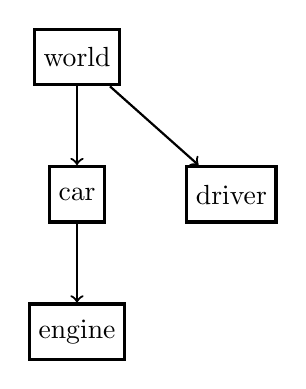
\begin{tikzpicture}[object/.style={rectangle, draw, very thick, minimum size=20}]
    \node[object] (World) {world};
    \node[object] (Car) [below=of World] {car};
    \node[object] (Driver) [right=of Car] {driver};
    \node[object] (Engine) [below=of Car] {engine};

    \draw[->,thick] (World) to (Car);
    \draw[->,thick] (World) to (Driver);
    \draw[->,thick] (Car) to (Engine);
  \end{tikzpicture}

  \caption{solid lines indicate "owns"}
\end{figure}
\end{frame}


\begin{frame}{Owners-as-dominators}
For \emph{a} to validly reference \emph{b}:
\begin{enumerate}
  \item \emph{a} is the owner of \emph{b},
  \item \emph{a} and \emph{b} are siblings, or
  \item \emph{b} is outside of \emph{a}.
\end{enumerate}

\begin{figure}[fragile]
  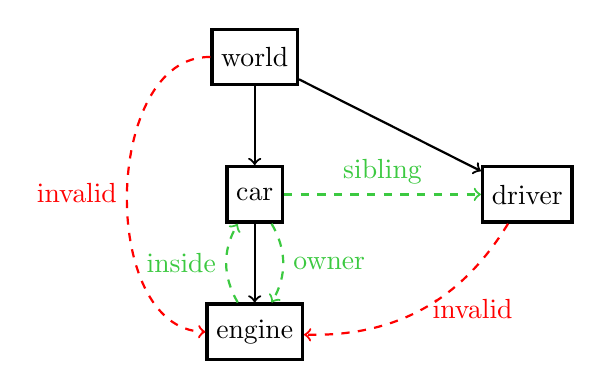
\begin{tikzpicture}[object/.style={rectangle, draw, very thick, minimum size=20}]
    \node[object] (World) {world};
    \node[object] (Car) [below=of World] {car};
    \node[object] (Driver) [right=of Car,xshift=1.5cm] {driver};
    \node[object] (Engine) [below=of Car] {engine};

    \draw[->,thick] (World) to (Car);
    \draw[->,thick] (World) to (Driver);
    \draw[->,thick] (Car) to (Engine);

    \draw[->,thick,dashed,cgreen] (Car) edge[bend left] node[right] {owner} (Engine);
    \draw[->,thick,dashed,cgreen] (Engine) edge[bend left] node[left] {inside} (Car);
    \draw[->,thick,dashed,cgreen] (Car) edge node[above] {sibling} (Driver);
    \draw[->,thick,dashed,red] (World) edge[bend right=90] node[left] {invalid} (Engine);
    \draw[->,thick,dashed,red] (Driver) edge[bend left] node[right] {invalid} (Engine);
  \end{tikzpicture}

  \caption{solid lines indicate "owns" and dotted lines indicate "references"}
\end{figure}
\end{frame}


\begin{frame}{Owners-as-dominators: implications}
\begin{itemize}
  \item any external reference to an object's internals must go through its owner
  \item objects are only protected from external access, not internal access
  % \item owners-as-dominators: owner is dominator for all of its owned objects
  \item model restricts \emph{where} references can point, not \emph{how} references are used
  \item doesn't allow common idioms that involve aliasing
\end{itemize}

\begin{figure}[fragile]
  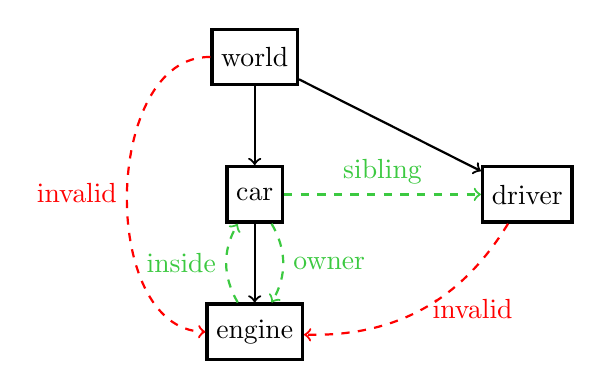
\begin{tikzpicture}[object/.style={rectangle, draw, very thick, minimum size=20}]
    \node[object] (World) {world};
    \node[object] (Car) [below=of World] {car};
    \node[object] (Driver) [right=of Car,xshift=1.5cm] {driver};
    \node[object] (Engine) [below=of Car] {engine};

    \draw[->,thick] (World) to (Car);
    \draw[->,thick] (World) to (Driver);
    \draw[->,thick] (Car) to (Engine);

    \draw[->,thick,dashed,cgreen] (Car) edge[bend left] node[right] {owner} (Engine);
    \draw[->,thick,dashed,cgreen] (Engine) edge[bend left] node[left] {inside} (Car);
    \draw[->,thick,dashed,cgreen] (Car) edge node[above] {sibling} (Driver);
    \draw[->,thick,dashed,red] (World) edge[bend right=90] node[left] {invalid} (Engine);
    \draw[->,thick,dashed,red] (Driver) edge[bend left] node[right] {invalid} (Engine);
  \end{tikzpicture}
\end{figure}
\end{frame}


\begin{frame}{Owners-as-modifiers}
Same rules as owners-as-dominators, but \emph{a} can also reference \emph{b} through \emph{r}, if:
\begin{enumerate}
  \item \emph{r} is a read-only reference and only pure methods (that don't modify existing objects) can be called on it.
\end{enumerate}

\begin{figure}
  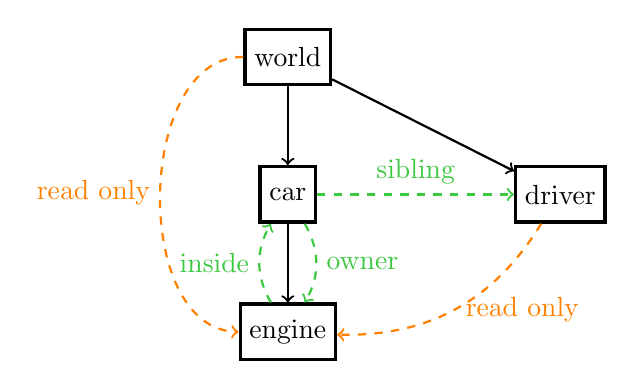
\begin{tikzpicture}[object/.style={rectangle, draw, very thick, minimum size=20}]
    \node[object] (World) {world};
    \node[object] (Car) [below=of World] {car};
    \node[object] (Driver) [right=of Car,xshift=1.5cm] {driver};
    \node[object] (Engine) [below=of Car] {engine};

    \draw[->,thick] (World) to (Car);
    \draw[->,thick] (World) to (Driver);
    \draw[->,thick] (Car) to (Engine);

    \draw[->,thick,dashed,cgreen] (Car) edge[bend left] node[right] {owner} (Engine);
    \draw[->,thick,dashed,cgreen] (Engine) edge[bend left] node[left] {inside} (Car);
    \draw[->,thick,dashed,cgreen] (Car) edge node[above] {sibling} (Driver);
    \draw[->,thick,dashed,orange] (World) edge[bend right=90] node[left] {read only} (Engine);
    \draw[->,thick,dashed,orange] (Driver) edge[bend left] node[right] {read only} (Engine);
  \end{tikzpicture}
\end{figure}
\end{frame}


\begin{frame}{Owners-as-modifiers: implications}
\begin{itemize}
  \item owners-as-modifiers: only the owners can modify objects
  \item model allows references to objects in arbitrary contexts, but restricts \emph{how} the references can be used
  % \item fulfills requirements for verification of the functional correctness of object-oriented programs
\end{itemize}

\begin{figure}
  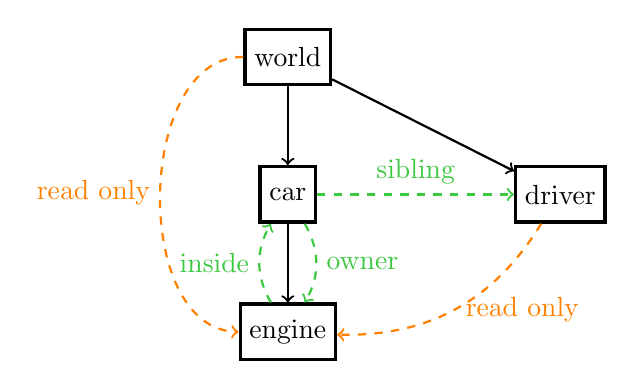
\begin{tikzpicture}[object/.style={rectangle, draw, very thick, minimum size=20}]
    \node[object] (World) {world};
    \node[object] (Car) [below=of World] {car};
    \node[object] (Driver) [right=of Car,xshift=1.5cm] {driver};
    \node[object] (Engine) [below=of Car] {engine};

    \draw[->,thick] (World) to (Car);
    \draw[->,thick] (World) to (Driver);
    \draw[->,thick] (Car) to (Engine);

    \draw[->,thick,dashed,cgreen] (Car) edge[bend left] node[right] {owner} (Engine);
    \draw[->,thick,dashed,cgreen] (Engine) edge[bend left] node[left] {inside} (Car);
    \draw[->,thick,dashed,cgreen] (Car) edge node[above] {sibling} (Driver);
    \draw[->,thick,dashed,orange] (World) edge[bend right=90] node[left] {read only} (Engine);
    \draw[->,thick,dashed,orange] (Driver) edge[bend left] node[right] {read only} (Engine);
  \end{tikzpicture}
\end{figure}
\end{frame}

\section{Ownership in Rust}

\begin{frame}[fragile]{From theory to implementation}
\begin{itemize}
  \item Rust's ownership system: extends owners-as-modifiers
  \begin{itemize}
    \item immutable (read-only) and mutable references % (not in owners-as-dominators)
    \item rules for compiler to check validity of references
  \end{itemize}

  \pause
  \item ownership rules in Rust:
  \begin{enumerate}
    \item Each value has an owner.
    \item There can only be one owner at a time.
    \item When the owner goes out of scope, the value will be \emph{dropped} (associated memory is freed).
  \end{enumerate}
  \begin{lstlisting}[language=Rust]
  { // a is not declared yet
    let a = 42; // scope of a starts here
    // do stuff with a
  } // scope is over => a is no longer valid
  \end{lstlisting}

  \pause
  \item Variables are immutable by default
  \begin{lstlisting}[language=Rust]
  let a = 42; // immutable
  a = 24; // invalid
  let mut b = 42; // mutable
  b = 24; // valid
  \end{lstlisting}
\end{itemize}
\end{frame}


% \begin{frame}{Memory allocation system}
% \end{frame}

% TODO: variable scope


\begin{frame}[fragile]{Transferring ownership}
Heap-based values: 
\begin{itemize}
  \item unknown size at compile time
  \item copying the value at runtime could be costly
  \item values are "moved" (between variables) by default

  \begin{lstlisting}[language=Rust]
  fn main() {
    let a = String::from("hello world");
    let b = a; // ownership transfer: a is moved into b
    println!("{}", a); // compiler error: a no longer valid
    let c = take_ownership(b); // b is moved into function
  }
  fn take_ownership(s: String) -> String {
    // do something with s
    String::from("new hello world")
  }
  \end{lstlisting}
  \item create deep copies with explicit \verb|clone()| call
\end{itemize}
\end{frame}


\begin{frame}[fragile]{Transferring ownership}
Stack-based primitives: 
\begin{itemize}
  \item examples: i32, u8, f64, char, bool etc.
  \item small, known size at compile time
  \item values are copied by default

  \begin{lstlisting}[language=Rust]
  let x: u32 = 42;
  let y: u32 = x; // x is copied instead of moved
  println!("x: {}, y: {}", x, y); // x and y valid
  \end{lstlisting}
  % \item stack-based values implement \verb|Copy| trait
\end{itemize}
\end{frame}


\begin{frame}[fragile]{Borrowing}
\begin{itemize}
  \item creating a reference in Rust is called \emph{borrowing}
  \item \emph{reference}: an address that points to a value that is owned by another variable
  \item unlike \emph{pointers}, a reference is guaranteed to point to a valid value
  % \item a reference does not own the value it points to $\rightarrow$ only reference (not the borrowed value) is dropped at the end of the reference's scope
  \item used for performing operations on values without taking ownership
  \item every reference has a \emph{lifetime}: scope for which reference is valid
  \item lifetime of borrowed value must be at least as long as lifetime of reference
  % \item a reference does not own the value it points to
  % \item the scope of a reference starts where it is introduced and extends until the last time it is used
  % \item Rust supports immutable (\verb|&|) and mutable (\verb|&mut|) references
\end{itemize}
\end{frame}


% \begin{frame}[fragile]{Lifetimes}
% \begin{itemize}
%   \item references grant temporary access to values $\rightarrow$ how long is "temporary"?
%   \item every reference has a \emph{lifetime}: scope for which reference is valid
%   \item \emph{borrow checker} uses lifetimes to ensure that all borrows are valid

%   % \item program is valid if all of the below hold for all references:
%   % \begin{enumerate}
%   %   \item the reference can only be used while its lifetime is ongoing
%   %   % \item the original referent is not used at all (for mutable references) or does not get mutated (for immutable references) until the lifetime of the newly created reference has expired.
%   %   \item immutable reference: the borrowed value does not get mutated during lifetime
%   %   \item mutable reference: the borrowed value is not used at all during lifetime
%   % \end{enumerate}

%   % \item lifetime annotations: \verb|&'a T| or \verb|&'a mut T| , where \verb|'a| is the lifetime of the reference
%   % \item compiler uses conventions to elide lifetimes $\rightarrow$ explicit annotations not always required
% \end{itemize}
% \end{frame}


\begin{frame}[fragile]{Borrowing: immutable references}
\begin{itemize}
  \item read-only/shared references $\rightarrow$ compiler disallows modifying borrowed value
  \item \verb|&| and \verb|*| operators
  \item borrow-checker rule: the borrowed value does not get mutated during lifetime
  \item unlimited amount of immutable references to same value (if no mutable references or mutations)

  \begin{lstlisting}[language=Rust]
  let s = String::from("hello");
  let r1 = &s; // 1. reference
  let r2 = &s; // 2. reference
  println!("r1: {}, r2: {}", *r1, *r2);
  \end{lstlisting}
\end{itemize}
\end{frame}


\begin{frame}[fragile]{Borrowing: mutable references}
\begin{itemize}
  \item borrowed value may be modified
  \item acquired using the \verb|&mut| keyword
  \item borrowed value must be mutable with \verb|mut| (variables are immutable by default)

  \begin{lstlisting}[language=Rust]
  let mut s = String::from("hello");
  s.push_str(" world");
  String::push_str(&mut s, " world"); // equivalent
  \end{lstlisting}
\end{itemize}
\end{frame}


\begin{frame}[fragile]{Borrowing: mutable references}
\begin{itemize}
  % \item \emph{data races}: multiple pointers access the same data simultaneously and at least one is writing to the data
  % \item goal: prevent \emph{data races} at compile time
  \item borrow-checker rule: the borrowed value is not used at all during lifetime
  % \item lifetime of mutable reference may not overlap with lifetime of any other (immutable or mutable) reference
  % \item only one mutable reference to a value allowed at any given time

  \begin{lstlisting}[language=Rust]
  let mut v = vec![10, 11];
  let vptr = &mut v[1];  // lifetime 'a starts
  Vec::push(&mut v, 12); // lifetime 'b starts and ends
  println!("{}", *vptr); // lifetime 'a ends
  \end{lstlisting}
  \pause
  \begin{lstlisting}[language=Rust]
  let mut v = vec![10, 11];
  Vec::push(&mut v, 12); // lifetime 'b starts and ends
  let vptr = &mut v[1];  // lifetime 'a starts
  println!("{}", *vptr); // lifetime 'a ends
  \end{lstlisting}
\end{itemize}
\end{frame}


\begin{frame}[fragile]{Borrowing: examples}
\begin{itemize}
  \begin{lstlisting}[language=Rust]
  let a;
  {
    let b: u32 = 42;
    a = &b;
  }
  println!("{}", *a) // dereference a
  \end{lstlisting}

  \item Will it compile? \pause No.
  \item Why not? Borrowed value 'b' does not live as long as the reference 'a'.
  \item Refactored version that compiles:\pause

  \begin{lstlisting}[language=Rust]
  let a;
  let b: u32 = 42;
  a = &b;
  println!("{}", *a) // dereference a
  \end{lstlisting}
\end{itemize}
\end{frame}


\begin{frame}[fragile]{Borrowing: examples}
\begin{itemize}
  \begin{lstlisting}[language=Rust]
  let mut s = String::from("hello world");
  let r = &s;
  s = String::from("hello world again");
  println!("{}", *r);
  \end{lstlisting}

  \item Will it compile? \pause No.
  \item Why not? Violated rule: the borrowed value does not get mutated during lifetime
  \item Refactored version that compiles:\pause

  \begin{lstlisting}[language=Rust]
  let mut s = String::from("hello world");
  s = String::from("hello world again");
  let r = &s;
  println!("{}", *r);
  \end{lstlisting}
\end{itemize}
\end{frame}


% \begin{frame}[fragile]{Borrowing: examples}
% \begin{itemize}
%   \begin{lstlisting}[language=Rust]
%   let mut s = String::from("hello");
%   let r1 = &s;
%   let r2 = &s;
%   println!("{} and {}", *r1, *r2);
%   let r3 = &mut s;
%   r3.push_str(" world");
%   \end{lstlisting}

%   \item Will it compile? \pause Yes.
%   \item Why? \pause Lifetimes of immutable and mutable references don't overlap.

%   \begin{lstlisting}[language=Rust]
%   let mut s = String::from("hello");
%   let r1 = &s; // lifetime r1 starts
%   let r2 = &s; // lifetime r2 starts
%   println!("{} and {}", *r1, *r2);
%   // lifetimes r1 and r2 end
%   let r3 = &mut s; // lifetime r3 starts
%   r3.push_str(" world");
%   \end{lstlisting}
% \end{itemize}
% \end{frame}


% \begin{frame}[fragile]{Borrowing: examples}
% \begin{itemize}
%   \begin{lstlisting}[language=Rust]
%   let mut s = String::from("hello");
%   let r = &s;
%   s.push_str(" world");
%   println!("{}", *r);
%   \end{lstlisting}

%   \item Will it compile? \pause No.
%   \item Why not? \pause Lifetimes of mutable and immutable references overlap (cannot borrow 's' as mutable because it is also borrowed as immutable)
%   \item Refactored version that compiles:\pause

%   \begin{lstlisting}[language=Rust]
%   let mut s = String::from("hello");
%   s.push_str(" world"); // lifetime starts and ends
%   let r = &s; // lifetime r starts
%   println!("{}", *r); // lifetime r ends
%   \end{lstlisting}
% \end{itemize}
% \end{frame}


\section{Evaluation}

\begin{frame}[fragile]{Another implementation: C++}
\begin{itemize}
  % \item integration of move semantics into language: Rust early on, C++ late in its life
  \item move semantics closely related to constructors and assignment operators (overloaded for classes)
  \item different reference types based on value categories:
  \begin{itemize}
    \item L-value references: refer to named values $\rightarrow$ copy
    \item R-value references: refer to temporary results of expression evaluations $\rightarrow$ move
  \end{itemize}
  \item \emph{overload resolution process} will select matching overload based on reference's value category
  \begin{lstlisting}[language=C++]
  struct S {
    S() {} // default constructor
    S(const S&) {...} // copy constructor
    S(S&&) {...} // move constructor
    S operator=(const S&) {...} // copy assignment operator
    S operator=(S&&) {... } // move assignment operator
    // ... more functions and data fields etc.
  }
  \end{lstlisting}
\end{itemize}
\end{frame}


\begin{frame}[fragile]{Move semantics: C++ vs Rust}
C++
\begin{lstlisting}[language=C++]
S s{};
S s_copied{s}; // copy constructor
S s_moved{std::move(s)}; // move constructor
// problem: 's' can still be used
\end{lstlisting}

\verb|std::move|:
\begin{itemize}
  \item "move" a named value by casting it to an R-value reference to tell compiler to use move constructor
  \item no formal effect on the lifetime of the moved-from object $\rightarrow$ moved-from object can still be used, but compiler can't guarantee it is valid
  \item no move constructor or move assignment operator implementation specification
\end{itemize}
\end{frame}


\begin{frame}[fragile]{Move semantics: C++ vs Rust}
C++
\begin{lstlisting}[language=C++]
S s{};
S s_copied{s}; // copy constructor
S s_moved{std::move(s)}; // move constructor
// problem: 's' can still be used
\end{lstlisting}

Rust
\begin{lstlisting}[language=Rust]
let s = S::default();
let s_copied = s.clone();
let s_moved = s; // 's' is moved
// compiler prevents use of 's'
\end{lstlisting}

Rust: safer move sematics through destructive moves enforced by the compiler
\end{frame}


\section{Conclusion}

\begin{frame}{Conclusions and outlook}
\begin{itemize}
  % \item programming languages based on ownership types can eliminate many aliasing-related issues by enforcing strict rules on the existence and behavior of references to values
  \item \emph{owners-as-dominators} and \emph{owners-as-modifiers} models: different strictness on \emph{where} and \emph{how} references may be used
  \item Rust: 
  \begin{itemize}
    \item ownership-related rules that are strictly enforced at compile time
    \item helpful compile-time error messages instead of crashes or UB at runtime
    % \item omitting the need for many manual, rigorous and error-prone memory reference checks that programmers used to have to perform
    % \item "fighting against the borrow checker" forces more explicit memory managenemt through ownership
  \end{itemize}
  \item will ownership types be incorporated into more new or existing programming languages in the future?
  \item maybe upcoming presentations on C++ enhancements (Carbon and cppfront) fix some of these issues?
\end{itemize}
\end{frame}


% \section{Extra slides}


\begin{frame}[fragile]{Lifetimes: example}
\begin{itemize}
  \begin{lstlisting}[language=Rust]
  fn main() {
    let s1 = String::from("short");
    let s2 = String::from("longest");
    let longest = longest(&s1, &s2);
    println!("longest string: '{}'", longest);
  }
  fn longest<'a>(s1: &'a str, s2: &'a str) -> &'a str {
    if s1.len() > s2.len() {
      s1
    } else {
      s2
    }
  }
  \end{lstlisting}
  \item longest function: return type contains a borrowed value, but unclear whether it is borrowed from 's1' or 's2'
  \item 's1' and 's2' have to live at least as long as lifetime 'a
\end{itemize}
\end{frame}


\begin{frame}[fragile]{Lifetime elision}
\begin{itemize}
  \item lifetime annotations: \verb|&'a T| or \verb|&'a mut T| , where \verb|'a| is the lifetime of the reference
  \item compiler uses conventions to elide lifetimes $\rightarrow$ explicit annotations not always required
  \item Here are the three rules:
  \begin{itemize}
    \item Each elided lifetime in a function’s arguments becomes a distinct lifetime parameter.
    \item If there is exactly one input lifetime, elided or not, that lifetime is assigned to all elided lifetimes in the return values of that function.
    \item If there are multiple input lifetimes, but one of them is &self or &mut self, the lifetime of self is assigned to all elided output lifetimes.
  \end{itemize}
  \item Otherwise, it is an error to elide an output lifetime.
\end{itemize}
\end{frame}


\begin{frame}[fragile]{Lifetime elision: examples}
\begin{lstlisting}[language=Rust]
fn print(s: &str); // elided
fn print<'a>(s: &'a str); // expanded

fn debug(lvl: u32, s: &str); // elided
fn debug<'a>(lvl: u32, s: &'a str); // expanded

fn substr(s: &str, until: u32) -> &str; // elided
fn substr<'a>(s: &'a str, until: u32) -> &'a str; // expanded

fn get_str() -> &str; // ILLEGAL, no inputs

fn frob(s: &str, t: &str) -> &str; // ILLEGAL, two inputs
fn frob<'a, 'b>(s: &'a str, t: &'b str) -> &str; // Expanded: Output lifetime is ambiguous
\end{lstlisting}
\end{frame}


\begin{frame}[fragile]{Borrow-checker rules}
  program is valid if all of the below hold for all references:
  \begin{enumerate}
    \item the reference can only be used while its lifetime is ongoing
    \item the original referent is not used at all (for mutable references) or does not get mutated (for immutable references) until the lifetime of the newly created reference has expired.
  \end{enumerate}
\end{frame}


\begin{frame}[fragile]{Formal lifetime rules}
\begin{itemize}
  \item Association rule:
  \begin{itemize}
    \item $x: \&'a T \;\Rightarrow\;scope(\text{x})\subseteq\text{'a}$
    \item A lifetime is a superset of the scope of its associated reference.}
  \end{itemize}

  \item Reference rule:
  \begin{itemize}
    \item $x: \&'a T = \&y \;\Rightarrow\;\text{'a}\subseteq scope(\text{y})$
    \item A lifetime associated with a reference is a subset of the scope of the referent object.
  \end{itemize}

  \item Assignment rule:
  \begin{itemize}
    \item $x: \&'a S = y: \&'b T \;\Rightarrow\;\text{'a}\subseteq\text{'b}$
    \item The lifetime associated with the assignee is a subset of the lifetime associated with the assigner.
  \end{itemize}
\end{itemize}
\end{frame}


\end{document}
